Monitoring the performance of a newly approved treatment is crucial, a process commonly referred to as \emph{post-marketing surveillance}~\citep{vlahovic2011postmarketing}. Nowadays, the U.S. Food and Drug Administration promotes the integration of observational data in this process to address the shortcomings of randomized evidence~\citep{platt2018fda,klonoff2020new}. This strategy is essential for validating personalized treatments, like immunotherapy for certain types of cancer, where randomized evidence is scarce, and treatment costs are substantial~\citep{hayden2016gene,goetz2018personalized}.

 Yet, unobserved confounding can significantly compromise causal conclusions drawn from observational data.  To tackle this issue, sensitivity analysis has been the prevalent paradigm since its conception by~\citet{cornfield59}.
 This field studies how a specific strength of unobserved confounding affects causal conclusions and introduces the concept of a \emph{critical value}~\citep{vanderweele2017sensitivity, jin2023sensitivity}, i.e. the minimum strength unobserved confounders would need to have to explain away the estimated treatment effect. However, critical values are solely based on observational data and can differ substantially from the \emph{true confounding strength}. As a result, epidemiologists often rely on heuristic judgments to decide whether an observational study is flawed.


Estimating the true confounding strength is infeasible without further assumptions.
Yet, once a treatment gains approval, we may have access to a randomized trial that allows for more effective strategies to address unobserved confounding. A recent line of works proposes to combine the estimators from randomized and observational data, e.g. see \citet{colnet2020causal,brantner2023methods} for a survey. However, these methods crucially rely on some prior knowledge of the confounding bias structure, that is not always available in practice. 
 
\begin{figure*}
    \centering 
    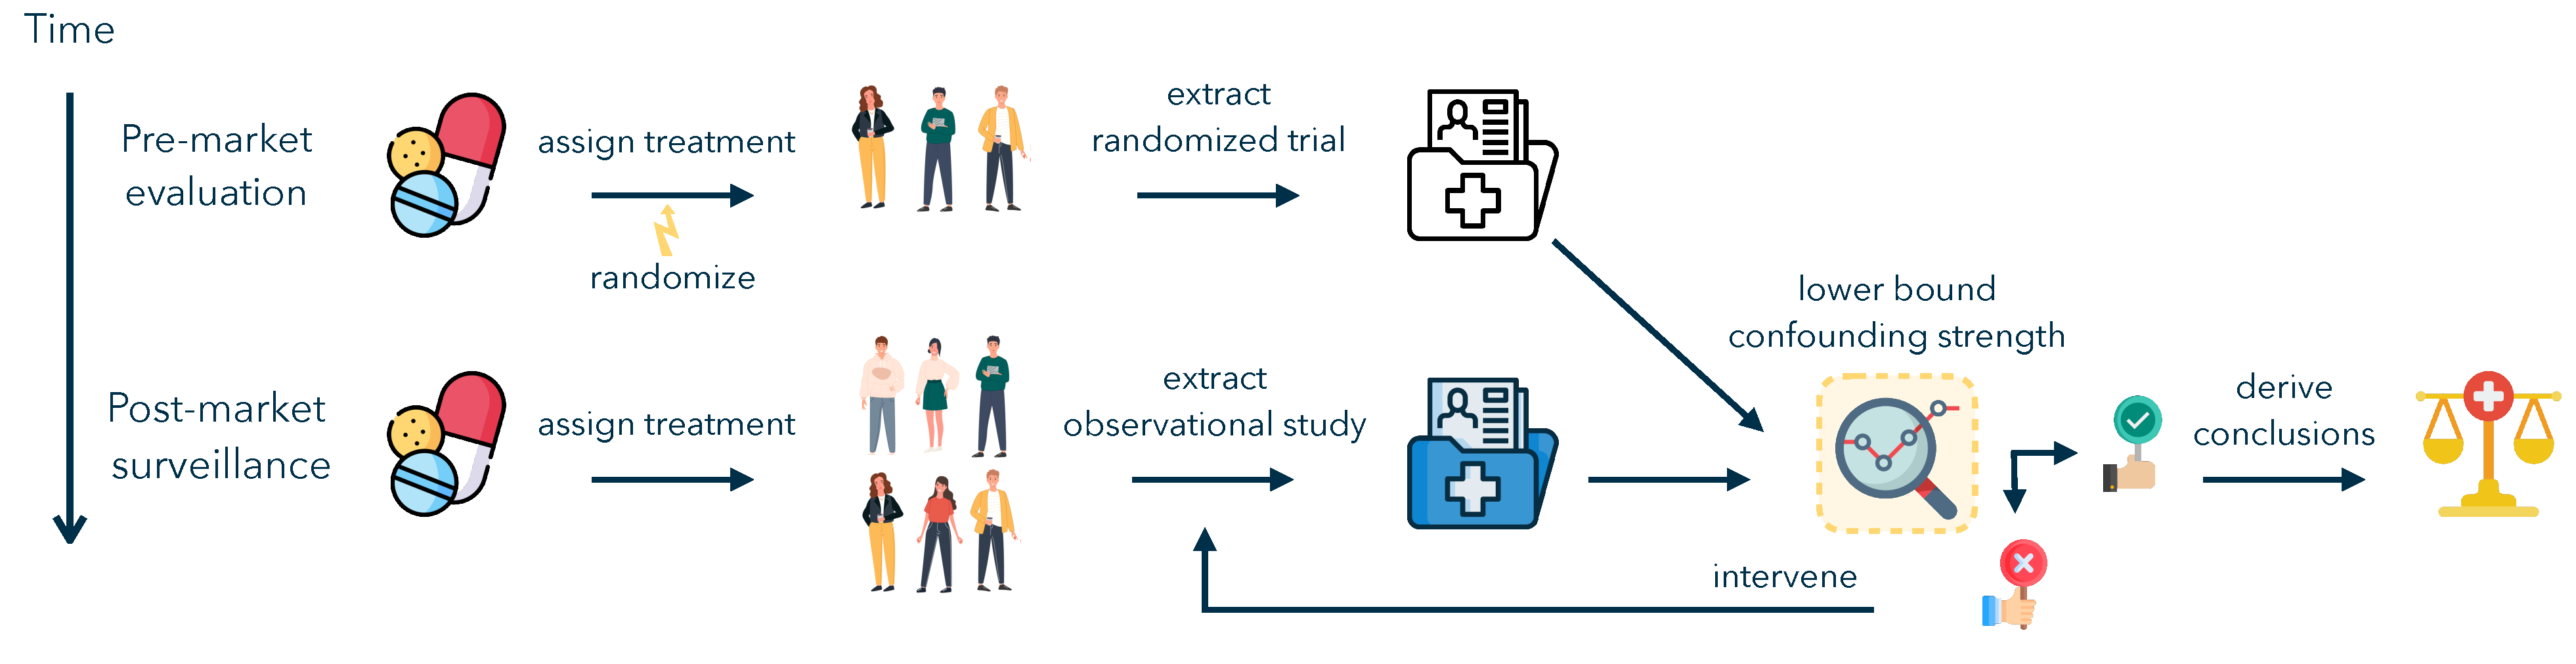
\includegraphics[width=\textwidth]{motivating_example} 
    \caption{An illustrative example of the drug regulatory process: our lower bound allows taking proactive measures to address the unobserved confounding problem.} 
    \label{fig:motivating_example} 
\end{figure*}


We propose an alternative strategy to leverage randomized trials, that is, to test and quantify the true confounding strength. In particular, if strong confounding is detected, epidemiologists can take proactive measures to correct it. Most directly, they can identify and incorporate relevant covariates into the study design if they were initially overlooked~\citep{dreyer2018advancing}. On the other hand, if small confounding is detected, epidemiologists can continue their analysis (see~\Cref{fig:motivating_example} for an illustration of the pipeline). More concretely, our contributions are as follows.
\begin{itemize}
\vspace{-2mm}
\item In~\Cref{sec:test}, we introduce the first statistical test to detect unobserved confounding above a certain strength. Further, we show how the test can be used to estimate an asymptotically valid lower bound on the true confounding strength.
\item In \Cref{sec:syn_exp}, we evaluate the finite-sample validity and power of our test on several synthetic and semi-synthetic datasets. 
\item In~\Cref{sec:whi_exp},
we showcase through a real-world example how our approach leads to conclusions that align with established epidemiological knowledge.
\end{itemize}


